%!TEX root=kdd15_workshop_main.tex
\section{Introduction}

% main point
We consider the problem of partitioning a streaming graph on a distributed memory system.
We are particularly interested in doing so for the kinds of irregular graphs that arise in applications like fraud detection, bioinformatics, and social and information network analysis, among numerous others.
%
%\subsection{Graph Partitioning}
%motivation: this is fluff; remove
\ignore{
From fraud detection to bioinformatics, large-scale graph mining and analytics provide access and deeper insight into the rich patterns in our data.
The availability and granularity of our network data is growing at an impressive pace.
With billions of online interactions, social networks (like e-commerce or the Twittersphere) have grown so immense and rich with data that they cannot easily be analyzed on a single machine.
Spreading these large graphs across multiple systems for analysis often takes complex algorithms with long computation times.
Modern data analytics moves fast, and the partitioning of massive graphs should too.
}
%
%Distributed, irregular algorithms such as large-scale graph mining often encounter bottlenecks in network communication and load imbalance~\cite{challenglums}.
The speed of mining algorithms on such graphs, at scale, is often limited by bottlenecks in network communication and load imbalance~\cite{challenglums}.
Partitioning is the common preprocessing step to find a mapping of the data to processors of the system that alleviates these two issues;
%Graph partitioning is the general problem of dividing a graph into separate components with desired properties;
in distributed computing the desired objective is generally the minimization of inter-partition edges (to minimize communication) subject to balanced partition size (to favor load balance).

Formally, we wish to partition the nodes of a graph into $k$ balanced components with capacity $(1+\epsilon)\frac{N}{k}$, such that the number of edges crossing partition boundaries is minimized. Partitioning with these two requirements can be reduced to the minimum-bisection problem~\cite{Garey:1979:CIG:578533} and is therefore NP-Complete. 
Thus, computing an optimal mapping is generally computationally infeasible, and heuristic approaches are taken. 

\begin{figure}[ht]
\centering
  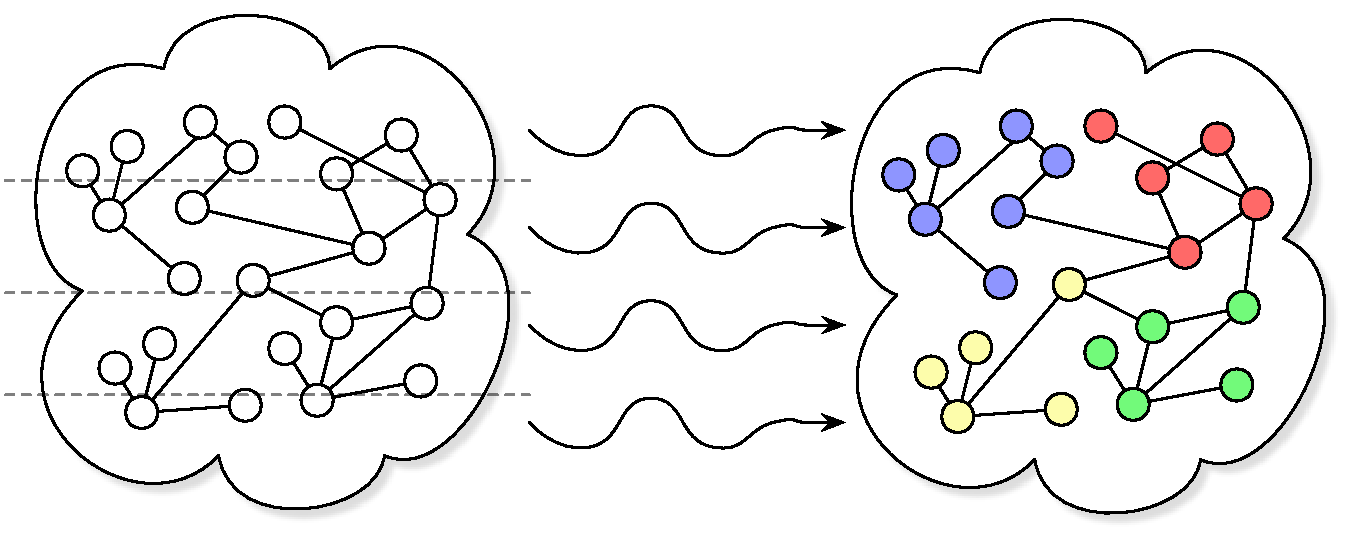
\includegraphics[width=0.7\columnwidth]{figures/coverfig.pdf}
  %\caption{Partition speed of various Kronecker graphs.}
  \label{fig:coverfig}
  \caption{Parallel streaming partitioning.}
\end{figure}

To illustrate the role of partitioning on performance, consider a parallel Breadth-First Search (BFS) where a graph's vertices are partitioned between two machines in a `1D' distribution~\cite{Buluc2D}. During each BFS step, each process must communicate all newly explored target vertices to process that owns them. In Figure~\ref{fig:0}, if we have 4 processes, all 14 nonzeros in the non-diagonal blocks must be communicated at some point. A good partitioner concentrates nonzeros in the diagonal blocks, thereby reducing communication.\footnote{Computing exact communication volume requires a hypergraph partitioner~\cite{hypergraph}.} 

% \todo{In the figure: Differentiate the cut-edges and their associated non-zeroes from the internal edges, to emphasize that they are undersirable.}
\begin{figure}[h]
\centering
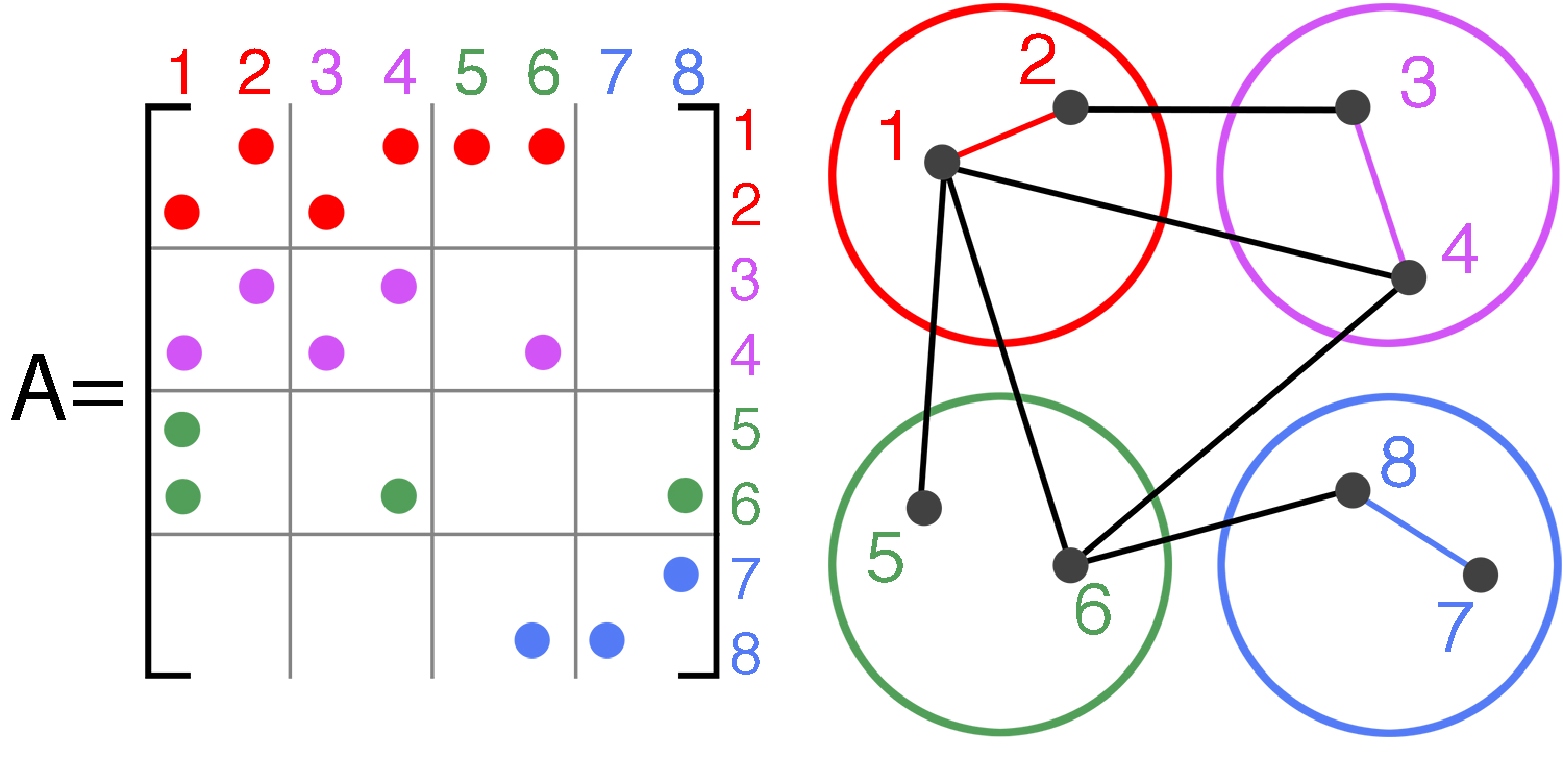
\includegraphics[width=0.85\columnwidth] {figures/graphpart1.pdf}
\caption[Caption for]{Graph 4-partition shown with corresponding adjacency matrix. The intra-partition edges are shown in their partition color, while inter-partition edges are shown in black.  Inter-partition edges result in additional network communication and lowered performance. }
\label{fig:0}
\end{figure}

Offline graph partitioning algorithms have existed for dec\-ades. They work by storing the graph in memory with complete information about the edges. Many variants of these algorithms exist~\cite{gpsurvey} and range from spatial methods~\cite{Gilbert95geometricmesh} to spectral methods~\cite{arora2009expander}. Some of the most effective offline graph partitioners are multi-level partitioners, which recursively contract the graph to a small number of vertices, and then heuristically optimize the partitioning while expanding back to the original graph~\cite{karypis1998multilevel}.
These methods are especially effective on geometric graphs, that is, graphs that arise from some physical geometry, like the discretized finite element mesh of a physical object.
Parallel multi-level partitioners will serve as the baseline comparison for our implementation. 

\paragraph{Streaming Partitioning}
Streaming partitioning is the process of partitioning a graph in a single sweep, reading vertices and edges only once. Thus we incur $O(|V| + |E|)$ memory access, storage, and run time, with minimal overhead. Offline graph partitioners require the whole graph to be represented in memory, whereas streaming graph partitioning can process vertices as they arrive. This fits a model where input data arrive sequentially from a generating source (such as a web-crawler).

Partitioning a \SI{26}{\giga\byte} Twitter graph has been shown to take \SI[abbreviations=false]{8}{\hours} using the fastest offline algorithms, and only \SI{40}{\minutes} with the FENNEL streaming partitioner, with similar partition quality~\cite{tsourakakis2012fennel}. This also suggests that we could do multiple, iterative passes of a streaming partitioner, all in a fraction of the time that an offline partitioner would take to terminate. This technique and its convergence properties have been explored by Nishimura and Ugander~\cite{nishimura2013restream}. In this paper we demonstrate empirically that distributing this streaming partitioning process can reduce the run-time for problem of this magnitude to a matter of \emph{seconds}. 

\paragraph{Contributions}
We have developed \ourmethod, a fast, iterative, distributed streaming graph partitioner.
It works by restreaming the distributed graph with tempered partition parameters to achieve a fast, parallel \textit{k}-partitioning.
We make the following contributions:
\begin{itemize}
\item A \textbf{scalable} distributed, open-source partitioner implementation using MPI.
\item Support for \textbf{streaming} and restreaming partitioning regardless of stream order.
\item A robust method for automatically tuning \ourmethod parameters 
\end{itemize}



